\documentclass[11pt]{article}
\usepackage{mathblatt}
% gesetzt von werkzeuge/setzer.py (Sorte selbst) aus dem Lernweg DXZ
% und den Bankzeilen; Muster bau/proben/2026-10-09/hypotenuse-muster.
\usepackage{enumitem}
\usepackage{adjustbox,varwidth}
\newgeometry{a4paper,margin=18mm,top=15mm,bottom=20mm,footskip=9mm}
\pagestyle{fancy}\fancyhf{}\renewcommand{\headrulewidth}{0pt}
\fancyfoot[L]{\footnotesize\color{mbgrau}DXZ \textperiodcentered{} Dezimalzahlen}
\fancyfoot[R]{\footnotesize\color{mbgrau}\thepage}
\setlength{\parskip}{3pt}
\renewcommand{\kreuz}[1]{\mbox{$\square$\ #1}\quad}
\newcommand{\kreuzl}[1]{\par\hangindent1.4em\hangafter1\noindent$\square$\ #1}
\newcommand{\aufg}[3]{\par\noindent\makebox[0pt][r]{#3}\begin{minipage}[t]{\linewidth}#1\end{minipage}\par}
\newcommand{\aufgg}[4]{\par\noindent\makebox[0pt][r]{#4}\begin{minipage}[t]{0.6\linewidth}\vspace{0pt}#1\end{minipage}\hfill
  \begin{minipage}[t]{0.37\linewidth}\vspace{0pt}\centering #2\end{minipage}\par}
\newcommand{\nr}[1]{\makebox[7mm][l]{\textbf{#1}}}
\newcommand{\lsg}[3]{\par\noindent\begin{minipage}[t]{9mm}\textbf{#1}\end{minipage}%
  \begin{minipage}[t]{52mm}\raggedright\bfseries\boldmath #2\end{minipage}\hspace{3mm}%
  \begin{minipage}[t]{\dimexpr\linewidth-64mm\relax}\raggedright\small #3\end{minipage}\par\vspace{4pt}}
\newlength{\kr}
\makeatletter
\newcommand{\karomerk}[2]{\protected@write\@auxout{}{\string\karoseite{#1}{#2}{\thepage}}}
\newcommand{\karoseite}[3]{\expandafter\xdef\csname karo@#1@#2\endcsname{#3}}
\newcommand{\karohinweis}[3]{\karomerk{h}{#1}\ifcsname karo@k@#1\endcsname
  \ifnum\csname karo@k@#1\endcsname=0\csname karo@h@#1\endcsname\relax#2\else#3\fi
  \else#3\fi}
\makeatother
\begin{document}

\noindent{\LARGE\bfseries Dezimalzahlen}\par\smallskip
\noindent{\small\color{mbgrau}Selbstlernheft Klasse 6 \textperiodcentered{} mit Lösungsheft \textperiodcentered{} Kennung DXZ}\par\medskip
\noindent\textbf{So nutzt du das Heft:} Lies im Abschnitt das Beispiel. Rechne dann die Aufgaben der Reihe nach und vergleiche jede sofort mit dem Lösungsheft. Kreuze „kann ich“ an, wenn du die letzte Aufgabe (\emph{Ziel}) allein schaffst.\par
\noindent Mehr Aufgaben zu einem Abschnitt: Kennung deinem Nachhilfelehrer schicken (z.\,B. „DXZ mehr B“).\par\medskip
{\arrayrulecolor{mbgrau}\renewcommand{\arraystretch}{1.3}
\noindent\begin{tabular}{|>{\bfseries}p{10mm}|p{112mm}|>{\raggedleft\arraybackslash}p{10mm}|>{\centering\arraybackslash}p{14mm}|}\hline
\rowcolor{black!8} & \textbf{Abschnitt} & \textbf{Seite} & \textbf{kann ich}\\\hline
A & Zehntel, Hundertstel, Tausendstel & \pageref{s:A} & $\square$\\\hline
B & Am Zahlenstrahl: ablesen, eintragen, weiterzählen & \pageref{s:B} & $\square$\\\hline
C & Bruch und Dezimalzahl: erweitern und kürzen & \pageref{s:C} & $\square$\\\hline
D & Teilen: Zähler durch Nenner, auch periodisch & \pageref{s:D} & $\square$\\\hline
T & Probetest & \pageref{s:T} & $\square$\\\hline
\end{tabular}}\par\bigskip

\begin{tcolorbox}[colback=mbkasten,colframe=mbgrau,boxrule=0.5pt,arc=1mm,left=3mm,right=3mm,top=2mm,bottom=2mm,title={\bfseries Formel auf einen Blick},coltitle=black,colbacktitle=black!10]
{\Large erweitern: $\dfrac{Z}{N} = \dfrac{Z \cdot k}{N \cdot k}$ \qquad kürzen: $\dfrac{Z}{N} = \dfrac{Z : k}{N : k}$}\par\medskip
In Worten: Erweitern und Kürzen ändern den Wert eines Bruchs nicht.\par\medskip
\end{tcolorbox}
\medskip\noindent\textbf{Typische Fehler – so nicht}\par\smallskip
\noindent\nr{$\times$}Bruchstrich als Komma gelesen: $\dfrac{1}{8}$ ist nicht $1{,}8$, sondern $1 : 8 = 0{,}125$.\par
\noindent\nr{$\times$}Nullen vergessen: $\dfrac{5}{100} = 0{,}05$, nicht $0{,}5$.\par
\clearpage\label{s:A}\noindent\colorbox{black!12}{\makebox[10mm]{\Large\bfseries\strut A}}\hspace{3mm}{\Large\bfseries Zehntel, Hundertstel, Tausendstel}\par\smallskip
\noindent Nach dem Komma kommen Zehntel, Hundertstel, Tausendstel; jede Stelle ist zehnmal kleiner als die davor. Ein \textbf{Zehnerbruch} (Nenner 10, 100, 1000) hat so viele Stellen nach dem Komma, wie sein Nenner Nullen hat – leere Stellen bekommen eine 0.\par\medskip
\noindent\textbf{Formel}\par\nopagebreak\noindent\hspace*{4mm}\begin{minipage}{\dimexpr\linewidth-4mm\relax}$\dfrac{7}{10} = 0{,}7$ \qquad $\dfrac{7}{100} = 0{,}07$ \qquad $\dfrac{7}{1000} = 0{,}007$ \qquad $\dfrac{347}{100} = 3{,}47$\end{minipage}\par\medskip
\noindent\textbf{Beispiel}\quad Schreibe $\dfrac{23}{1000}$ als Dezimalzahl und trage sie in die Stellenwerttafel ein.\par\smallskip
\noindent\begin{minipage}[t]{0.6\linewidth}\vspace{0pt}\par\noindent\hangindent6mm\hangafter1\makebox[6mm][l]{\textbf{1}}Der Nenner 1000 hat 3 Nullen: Die Zahl hat 3 Stellen nach dem Komma.\par\smallskip\par\noindent\hangindent6mm\hangafter1\makebox[6mm][l]{\textbf{2}}23 Tausendstel: Die 3 kommt in die Tausendstel-Spalte, die 2 in die Hundertstel-Spalte.\par\smallskip\par\noindent\hangindent6mm\hangafter1\makebox[6mm][l]{\textbf{3}}Leere Spalten bekommen eine 0: 0 Zehntel, 0 Einer.\par\smallskip\par\noindent\hangindent6mm\hangafter1\makebox[6mm][l]{\textbf{4}}Also $\dfrac{23}{1000} = 0{,}023$.\par\smallskip\end{minipage}\hfill
\begin{minipage}[t]{0.37\linewidth}\vspace{0pt}\centering \adjustbox{max width=\linewidth}{\begin{varwidth}{50cm}\sachtabelle{cccc}{Einer & Zehntel & Hundertstel & Tausendstel}{0 & 0 & 2 & 3}\end{varwidth}}\end{minipage}\par\medskip
\noindent\textbf{Aufgaben}\hspace{1em}{\small\color{mbgrau}\karohinweis{A}{Rechne unten im Karo.}{Rechne auf einem extra Blatt.} Vergleiche jede Aufgabe gleich mit dem Lösungsheft.}\par\smallskip
\aufg{\hangindent7mm\hangafter1\nr{1.}Schreibe als Dezimalzahl. \par\vspace{3pt} a)~$\dfrac{3}{10}$ \qquad b)~$\dfrac{9}{10}$ \qquad c)~$\dfrac{47}{100}$ \qquad d)~$\dfrac{81}{100}$}{}{}
\medskip
\aufg{\hangindent7mm\hangafter1\nr{2.}Schreibe als Dezimalzahl. \par\vspace{3pt} a)~$\dfrac{6}{100}$ \qquad b)~$\dfrac{6}{1000}$ \qquad c)~$\dfrac{52}{1000}$ \qquad d)~$\dfrac{9}{100}$}{}{}
\medskip
\aufgg{\hangindent7mm\hangafter1\nr{3.}Welche Zahl zeigt die Stellenwerttafel? Schreibe sie als Dezimalzahl und als Zehnerbruch.}{\adjustbox{max width=\linewidth}{\begin{varwidth}{50cm}\sachtabelle{cccc}{Einer & Zehntel & Hundertstel & Tausendstel}{4 & 0 & 5 & 8}\end{varwidth}}}{}{}
\medskip
\aufg{\hangindent7mm\hangafter1\nr{4.}Schreibe als Zehnerbruch. \par\vspace{3pt} a)~$0{,}7$ \qquad b)~$0{,}13$ \qquad c)~$0{,}08$ \qquad d)~$2{,}019$}{}{}
\medskip
\aufg{\hangindent7mm\hangafter1\nr{5.}Beim Sportfest läuft Ben die 100\,m in 12 Sekunden und 7 Hundertsteln, Ali in 12 Sekunden und 7 Zehnteln. Welche Anzeige zeigt Bens Zeit? Kreuze an. Wer war schneller?\par\smallskip\leftskip7mm \kreuz{12{,}7\,s}\ \kreuz{12{,}07\,s}\par\kreuz{12{,}007\,s}\ \kreuz{1{,}207\,s}}{}{{\scriptsize\color{mbgrau}Ziel\hspace{2mm}}}
\medskip
\par\vspace{3mm}\setlength{\kr}{\dimexpr\pagegoal-\pagetotal-10mm\relax}%
\ifdim\kr>12mm\karomerk{k}{A}\noindent{\scriptsize\color{mbgrau}Platz zum Rechnen}\par\nointerlineskip\vspace{1mm}\noindent
\begin{tikzpicture}\clip (0,0) rectangle ({\linewidth-0.5mm},\kr);\draw[black!16,line width=0.3pt,step=5mm] (0,0) grid (\linewidth,\kr);\end{tikzpicture}\fi\par
\clearpage\label{s:B}\noindent\colorbox{black!12}{\makebox[10mm]{\Large\bfseries\strut B}}\hspace{3mm}{\Large\bfseries Am Zahlenstrahl: ablesen, eintragen, weiterzählen}\par\smallskip
\noindent Bestimme zuerst, wie groß ein Schritt ist: Zwischen zwei Einern liegen 10 Zehntel-Schritte, zwischen zwei Zehnteln 10 Hundertstel-Schritte. Zehn Zehntel sind ein Einer: Nach $2{,}9$ kommt $3{,}0$.\par\medskip
\noindent\textbf{Formel}\par\nopagebreak\noindent\hspace*{4mm}\begin{minipage}{\dimexpr\linewidth-4mm\relax}Schritt $=$ Abstand zweier beschrifteter Striche $:$ Zahl der Schritte \par\vspace{4pt} $4{,}37$ liegt zwischen den Zehnteln $4{,}3$ und $4{,}4$.\end{minipage}\par\medskip
\noindent\textbf{Beispiel}\quad Lies $A$ ab. Trage $2{,}35$ ein.\par\smallskip
\noindent\begin{minipage}[t]{0.6\linewidth}\vspace{0pt}\par\noindent\hangindent6mm\hangafter1\makebox[6mm][l]{\textbf{1}}Von 2 bis 3 sind es 10 Schritte: Ein Schritt ist $0{,}1$.\par\smallskip\par\noindent\hangindent6mm\hangafter1\makebox[6mm][l]{\textbf{2}}$A$ liegt 6 Schritte hinter 2: $A = 2{,}6$.\par\smallskip\par\noindent\hangindent6mm\hangafter1\makebox[6mm][l]{\textbf{3}}$2{,}35$ hat 3 Zehntel: Es liegt hinter $2{,}3$, vor $2{,}4$.\par\smallskip\par\noindent\hangindent6mm\hangafter1\makebox[6mm][l]{\textbf{4}}5 Hundertstel sind ein halber Zehntel-Schritt: genau in der Mitte.\par\smallskip\end{minipage}\hfill
\begin{minipage}[t]{0.37\linewidth}\vspace{0pt}\centering 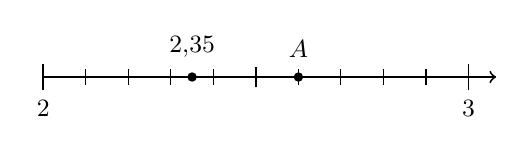
\begin{tikzpicture}[font=\small]\draw[->,line width=0.7pt] (0,0) -- (5.75,0);\draw[line width=0.7pt] (0.000,-0.17) -- (0.000,0.17);\node[below] at (0.000,-0.17) {$2$};\draw[line width=0.4pt] (0.540,-0.1) -- (0.540,0.1);\draw[line width=0.4pt] (1.080,-0.1) -- (1.080,0.1);\draw[line width=0.4pt] (1.620,-0.1) -- (1.620,0.1);\draw[line width=0.4pt] (2.160,-0.1) -- (2.160,0.1);\draw[line width=0.5pt] (2.700,-0.13) -- (2.700,0.13);\draw[line width=0.4pt] (3.240,-0.1) -- (3.240,0.1);\draw[line width=0.4pt] (3.780,-0.1) -- (3.780,0.1);\draw[line width=0.4pt] (4.320,-0.1) -- (4.320,0.1);\draw[line width=0.4pt] (4.860,-0.1) -- (4.860,0.1);\draw[line width=0.7pt] (5.400,-0.17) -- (5.400,0.17);\node[below] at (5.400,-0.17) {$3$};\fill (3.240,0) circle (1.7pt);\node[above] at (3.240,0.12) {$A$};\fill (1.890,0) circle (1.7pt);\node[above] at (1.890,0.12) {$2{,}35$};\end{tikzpicture}\end{minipage}\par\medskip
\noindent\textbf{Aufgaben}\hspace{1em}{\small\color{mbgrau}\karohinweis{B}{Rechne unten im Karo.}{Rechne auf einem extra Blatt.} Vergleiche jede Aufgabe gleich mit dem Lösungsheft.}\par\smallskip
\aufgg{\hangindent7mm\hangafter1\nr{1.}Welche Zahlen gehören zu $A$, $B$ und $C$?}{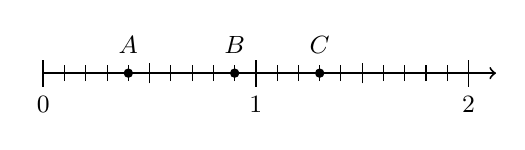
\begin{tikzpicture}[font=\small]\draw[->,line width=0.7pt] (0,0) -- (5.75,0);\draw[line width=0.7pt] (0.000,-0.17) -- (0.000,0.17);\node[below] at (0.000,-0.17) {$0$};\draw[line width=0.4pt] (0.270,-0.1) -- (0.270,0.1);\draw[line width=0.4pt] (0.540,-0.1) -- (0.540,0.1);\draw[line width=0.4pt] (0.810,-0.1) -- (0.810,0.1);\draw[line width=0.4pt] (1.080,-0.1) -- (1.080,0.1);\draw[line width=0.5pt] (1.350,-0.13) -- (1.350,0.13);\draw[line width=0.4pt] (1.620,-0.1) -- (1.620,0.1);\draw[line width=0.4pt] (1.890,-0.1) -- (1.890,0.1);\draw[line width=0.4pt] (2.160,-0.1) -- (2.160,0.1);\draw[line width=0.4pt] (2.430,-0.1) -- (2.430,0.1);\draw[line width=0.7pt] (2.700,-0.17) -- (2.700,0.17);\node[below] at (2.700,-0.17) {$1$};\draw[line width=0.4pt] (2.970,-0.1) -- (2.970,0.1);\draw[line width=0.4pt] (3.240,-0.1) -- (3.240,0.1);\draw[line width=0.4pt] (3.510,-0.1) -- (3.510,0.1);\draw[line width=0.4pt] (3.780,-0.1) -- (3.780,0.1);\draw[line width=0.5pt] (4.050,-0.13) -- (4.050,0.13);\draw[line width=0.4pt] (4.320,-0.1) -- (4.320,0.1);\draw[line width=0.4pt] (4.590,-0.1) -- (4.590,0.1);\draw[line width=0.4pt] (4.860,-0.1) -- (4.860,0.1);\draw[line width=0.4pt] (5.130,-0.1) -- (5.130,0.1);\draw[line width=0.7pt] (5.400,-0.17) -- (5.400,0.17);\node[below] at (5.400,-0.17) {$2$};\fill (1.080,0) circle (1.7pt);\node[above] at (1.080,0.12) {$A$};\fill (2.430,0) circle (1.7pt);\node[above] at (2.430,0.12) {$B$};\fill (3.510,0) circle (1.7pt);\node[above] at (3.510,0.12) {$C$};\end{tikzpicture}}{}{}
\medskip
\aufgg{\hangindent7mm\hangafter1\nr{2.}Hier ist ein Schritt ein Hundertstel. Trage $0{,}43$, $0{,}49$ und $0{,}56$ ein.}{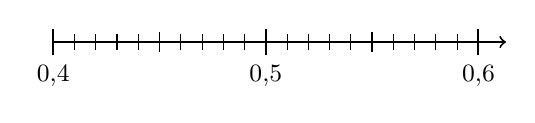
\begin{tikzpicture}[font=\small]\draw[->,line width=0.7pt] (0,0) -- (5.75,0);\draw[line width=0.7pt] (0.000,-0.17) -- (0.000,0.17);\node[below] at (0.000,-0.17) {$0{,}4$};\draw[line width=0.4pt] (0.270,-0.1) -- (0.270,0.1);\draw[line width=0.4pt] (0.540,-0.1) -- (0.540,0.1);\draw[line width=0.4pt] (0.810,-0.1) -- (0.810,0.1);\draw[line width=0.4pt] (1.080,-0.1) -- (1.080,0.1);\draw[line width=0.5pt] (1.350,-0.13) -- (1.350,0.13);\draw[line width=0.4pt] (1.620,-0.1) -- (1.620,0.1);\draw[line width=0.4pt] (1.890,-0.1) -- (1.890,0.1);\draw[line width=0.4pt] (2.160,-0.1) -- (2.160,0.1);\draw[line width=0.4pt] (2.430,-0.1) -- (2.430,0.1);\draw[line width=0.7pt] (2.700,-0.17) -- (2.700,0.17);\node[below] at (2.700,-0.17) {$0{,}5$};\draw[line width=0.4pt] (2.970,-0.1) -- (2.970,0.1);\draw[line width=0.4pt] (3.240,-0.1) -- (3.240,0.1);\draw[line width=0.4pt] (3.510,-0.1) -- (3.510,0.1);\draw[line width=0.4pt] (3.780,-0.1) -- (3.780,0.1);\draw[line width=0.5pt] (4.050,-0.13) -- (4.050,0.13);\draw[line width=0.4pt] (4.320,-0.1) -- (4.320,0.1);\draw[line width=0.4pt] (4.590,-0.1) -- (4.590,0.1);\draw[line width=0.4pt] (4.860,-0.1) -- (4.860,0.1);\draw[line width=0.4pt] (5.130,-0.1) -- (5.130,0.1);\draw[line width=0.7pt] (5.400,-0.17) -- (5.400,0.17);\node[below] at (5.400,-0.17) {$0{,}6$};\end{tikzpicture}}{}{}
\medskip
\aufg{\hangindent7mm\hangafter1\nr{3.}Zwischen welchen beiden Zehnteln liegt die Zahl? \par\vspace{3pt} a)~$3{,}46$ \qquad b)~$0{,}72$ \qquad c)~$5{,}09$ \qquad d)~$1{,}98$}{}{}
\medskip
\aufg{\hangindent7mm\hangafter1\nr{4.}Zähle drei Zahlen weiter. \par\vspace{3pt} a)~in $0{,}1$er-Schritten: $2{,}7$; $2{,}8$; … \par b)~in $0{,}2$er-Schritten: $0{,}6$; $0{,}8$; … \par c)~in $0{,}01$er-Schritten: $4{,}97$; $4{,}98$; …}{}{}
\medskip
\aufg{\hangindent7mm\hangafter1\nr{5.}Am Rand der Weitsprunggrube ist alle 10\,cm ein Strich. Mila springt $3{,}46$\,m. Zwischen welchen beiden Strichen landet sie? Welcher Strich ist näher?}{}{{\scriptsize\color{mbgrau}Ziel\hspace{2mm}}}
\medskip
\par\vspace{3mm}\setlength{\kr}{\dimexpr\pagegoal-\pagetotal-10mm\relax}%
\ifdim\kr>12mm\karomerk{k}{B}\noindent{\scriptsize\color{mbgrau}Platz zum Rechnen}\par\nointerlineskip\vspace{1mm}\noindent
\begin{tikzpicture}\clip (0,0) rectangle ({\linewidth-0.5mm},\kr);\draw[black!16,line width=0.3pt,step=5mm] (0,0) grid (\linewidth,\kr);\end{tikzpicture}\fi\par
\clearpage\label{s:C}\noindent\colorbox{black!12}{\makebox[10mm]{\Large\bfseries\strut C}}\hspace{3mm}{\Large\bfseries Bruch und Dezimalzahl: erweitern und kürzen}\par\smallskip
\noindent Lässt sich der Nenner auf 10, 100 oder 1000 erweitern, wird der Bruch ein Zehnerbruch – den schreibst du wie in A. Umgekehrt schreibst du die Dezimalzahl als Zehnerbruch und kürzt.\par\medskip
\noindent\textbf{Formel}\par\nopagebreak\noindent\hspace*{4mm}\begin{minipage}{\dimexpr\linewidth-4mm\relax}Nenner 2, 5 $\to$ 10 \qquad Nenner 4, 20, 25, 50 $\to$ 100 \par\vspace{4pt} $\dfrac{3}{4} = \dfrac{75}{100} = 0{,}75$ \qquad $0{,}6 = \dfrac{6}{10} = \dfrac{3}{5}$\end{minipage}\par\medskip
\noindent\textbf{Beispiel}\quad Schreibe $\dfrac{7}{20}$ als Dezimalzahl. Schreibe dann $0{,}35$ zurück als gekürzten Bruch.\par\smallskip
\noindent\par\noindent\hangindent6mm\hangafter1\makebox[6mm][l]{\textbf{1}}Welcher Zehnerbruch passt? $20 \cdot 5 = 100$: auf Hundertstel.\par\smallskip\par\noindent\hangindent6mm\hangafter1\makebox[6mm][l]{\textbf{2}}Mit 5 erweitern: $\dfrac{7}{20} = \dfrac{7 \cdot 5}{20 \cdot 5} = \dfrac{35}{100}$\par\smallskip\par\noindent\hangindent6mm\hangafter1\makebox[6mm][l]{\textbf{3}}35 Hundertstel: $\dfrac{35}{100} = 0{,}35$.\par\smallskip\par\noindent\hangindent6mm\hangafter1\makebox[6mm][l]{\textbf{4}}Zurück: $0{,}35 = \dfrac{35}{100}$, mit 5 kürzen: $\dfrac{7}{20}$.\par\smallskip\par\medskip
\noindent\textbf{Aufgaben}\hspace{1em}{\small\color{mbgrau}\karohinweis{C}{Rechne unten im Karo.}{Rechne auf einem extra Blatt.} Vergleiche jede Aufgabe gleich mit dem Lösungsheft.}\par\smallskip
\aufg{\hangindent7mm\hangafter1\nr{1.}Erweitere auf Zehntel und schreibe als Dezimalzahl. \par\vspace{3pt} a)~$\dfrac{1}{2}$ \qquad b)~$\dfrac{3}{5}$ \qquad c)~$\dfrac{4}{5}$ \qquad d)~$\dfrac{3}{2}$}{}{}
\medskip
\aufg{\hangindent7mm\hangafter1\nr{2.}Erweitere auf Hundertstel und schreibe als Dezimalzahl. \par\vspace{3pt} a)~$\dfrac{3}{4}$ \qquad b)~$\dfrac{9}{20}$ \qquad c)~$\dfrac{6}{25}$ \qquad d)~$\dfrac{7}{50}$}{}{}
\medskip
\aufg{\hangindent7mm\hangafter1\nr{3.}Schreibe als Zehnerbruch und kürze so weit wie möglich. \par\vspace{3pt} a)~$0{,}4$ \qquad b)~$0{,}25$ \qquad c)~$0{,}65$ \qquad d)~$1{,}2$}{}{}
\medskip
\aufg{\hangindent7mm\hangafter1\nr{4.}Welche Zahlen sind gleich groß? Schreibe je einen Bruch und die passende Dezimalzahl als Paar auf. \par\vspace{3pt} $\dfrac{3}{5}$ \qquad $\dfrac{7}{20}$ \qquad $\dfrac{1}{4}$ \qquad $\dfrac{2}{25}$ \par\vspace{6pt} $0{,}25$ \qquad $0{,}08$ \qquad $0{,}6$ \qquad $0{,}35$}{}{}
\medskip
\aufg{\hangindent7mm\hangafter1\nr{5.}Frau Kaya möchte drei Viertel Kilogramm Hackfleisch kaufen. Die Waage zeigt $0{,}7$\,kg. Wie viel Gramm fehlen noch? (1\,kg $= 1000$\,g)}{}{{\scriptsize\color{mbgrau}Ziel\hspace{2mm}}}
\medskip
\par\vspace{3mm}\setlength{\kr}{\dimexpr\pagegoal-\pagetotal-10mm\relax}%
\ifdim\kr>12mm\karomerk{k}{C}\noindent{\scriptsize\color{mbgrau}Platz zum Rechnen}\par\nointerlineskip\vspace{1mm}\noindent
\begin{tikzpicture}\clip (0,0) rectangle ({\linewidth-0.5mm},\kr);\draw[black!16,line width=0.3pt,step=5mm] (0,0) grid (\linewidth,\kr);\end{tikzpicture}\fi\par
\clearpage\label{s:D}\noindent\colorbox{black!12}{\makebox[10mm]{\Large\bfseries\strut D}}\hspace{3mm}{\Large\bfseries Teilen: Zähler durch Nenner, auch periodisch}\par\smallskip
\noindent Passt kein Zehnerbruch, teilst du den Zähler durch den Nenner; geht es nicht auf, hängst du hinter dem Komma Nullen an. Kommt derselbe Rest immer wieder, wiederholen sich die Ziffern ohne Ende: Die Zahl ist \textbf{periodisch} und bekommt einen Strich.\par\medskip
\noindent\textbf{Formel}\par\nopagebreak\noindent\hspace*{4mm}\begin{minipage}{\dimexpr\linewidth-4mm\relax}$\dfrac{Z}{N} = Z : N$ \qquad $\dfrac{1}{3} = 0{,}333\ldots = 0{,}\overline{3}$ \par\vspace{4pt} Strich nur über die Ziffern, die sich wiederholen: $\dfrac{1}{6} = 0{,}1666\ldots = 0{,}1\overline{6}$\end{minipage}\par\medskip
\noindent\textbf{Beispiel}\quad Schreibe $\dfrac{3}{8}$ als Dezimalzahl.\par\smallskip
\noindent\par\noindent\hangindent6mm\hangafter1\makebox[6mm][l]{\textbf{1}}8 lässt sich nicht bequem auf 10 oder 100 bringen: rechne $3 : 8$.\par\smallskip\par\noindent\hangindent6mm\hangafter1\makebox[6mm][l]{\textbf{2}}$3 : 8 = 0$, Rest 3. Schreibe 0 und das Komma.\par\smallskip\par\noindent\hangindent6mm\hangafter1\makebox[6mm][l]{\textbf{3}}Hänge eine 0 an: $30 : 8 = 3$, Rest 6. \quad $60 : 8 = 7$, Rest 4.\par\smallskip\par\noindent\hangindent6mm\hangafter1\makebox[6mm][l]{\textbf{4}}$40 : 8 = 5$, Rest 0 – fertig: $\dfrac{3}{8} = 0{,}375$.\par\smallskip\par\medskip
\noindent\textbf{Aufgaben}\hspace{1em}{\small\color{mbgrau}\karohinweis{D}{Rechne unten im Karo.}{Rechne auf einem extra Blatt.} Vergleiche jede Aufgabe gleich mit dem Lösungsheft.}\par\smallskip
\aufg{\hangindent7mm\hangafter1\nr{1.}Teile Zähler durch Nenner. \par\vspace{3pt} a)~$\dfrac{1}{4}$ \qquad b)~$\dfrac{3}{4}$ \qquad c)~$\dfrac{1}{8}$ \qquad d)~$\dfrac{7}{8}$}{}{}
\medskip
\aufg{\hangindent7mm\hangafter1\nr{2.}Der Bruch ist größer als 1. Teile Zähler durch Nenner. \par\vspace{3pt} a)~$\dfrac{9}{4}$ \qquad b)~$\dfrac{11}{8}$ \qquad c)~$\dfrac{21}{8}$}{}{}
\medskip
\aufg{\hangindent7mm\hangafter1\nr{3.}Teile Zähler durch Nenner. Die Division geht nicht auf: Schreib mit Strich. \par\vspace{3pt} a)~$\dfrac{1}{3}$ \qquad b)~$\dfrac{2}{3}$ \qquad c)~$\dfrac{5}{9}$ \qquad d)~$\dfrac{1}{6}$}{}{}
\medskip
\aufg{\hangindent7mm\hangafter1\nr{4.}Geht die Division auf? Schreibe ja oder nein. \par\vspace{3pt} a)~$\dfrac{3}{8}$ \qquad b)~$\dfrac{7}{20}$ \qquad c)~$\dfrac{5}{6}$ \qquad d)~$\dfrac{9}{25}$}{}{}
\medskip
\aufg{\hangindent7mm\hangafter1\nr{5.}Ein Band ist 5\,m lang. Es wird in 8 gleich lange Stücke geschnitten. Für eine Schleife braucht man 60\,cm. Reicht ein Stück für eine Schleife?}{}{{\scriptsize\color{mbgrau}Ziel\hspace{2mm}}}
\medskip
\par\vspace{3mm}\setlength{\kr}{\dimexpr\pagegoal-\pagetotal-10mm\relax}%
\ifdim\kr>12mm\karomerk{k}{D}\noindent{\scriptsize\color{mbgrau}Platz zum Rechnen}\par\nointerlineskip\vspace{1mm}\noindent
\begin{tikzpicture}\clip (0,0) rectangle ({\linewidth-0.5mm},\kr);\draw[black!16,line width=0.3pt,step=5mm] (0,0) grid (\linewidth,\kr);\end{tikzpicture}\fi\par
\clearpage\label{s:T}\noindent\colorbox{black!12}{\makebox[10mm]{\Large\bfseries\strut T}}\hspace{3mm}{\Large\bfseries Probetest}\par\smallskip
\noindent Gemischt, ohne Beispiel. Etwa 20 Minuten.\par\medskip
\noindent\textbf{Aufgaben}\hspace{1em}{\small\color{mbgrau}\karohinweis{T}{Rechne unten im Karo.}{Rechne auf einem extra Blatt.} Vergleiche jede Aufgabe gleich mit dem Lösungsheft.}\par\smallskip
\aufg{\hangindent7mm\hangafter1\nr{1.}Schreibe als Dezimalzahl. \par\vspace{3pt} a)~$\dfrac{9}{10}$ \qquad b)~$\dfrac{9}{100}$ \qquad c)~$\dfrac{45}{1000}$}{}{}
\medskip
\aufgg{\hangindent7mm\hangafter1\nr{2.}Welche Zahlen gehören zu $A$ und $B$? Zwischen welchen beiden Zehnteln liegt $A$?}{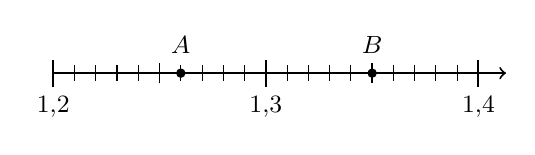
\begin{tikzpicture}[font=\small]\draw[->,line width=0.7pt] (0,0) -- (5.75,0);\draw[line width=0.7pt] (0.000,-0.17) -- (0.000,0.17);\node[below] at (0.000,-0.17) {$1{,}2$};\draw[line width=0.4pt] (0.270,-0.1) -- (0.270,0.1);\draw[line width=0.4pt] (0.540,-0.1) -- (0.540,0.1);\draw[line width=0.4pt] (0.810,-0.1) -- (0.810,0.1);\draw[line width=0.4pt] (1.080,-0.1) -- (1.080,0.1);\draw[line width=0.5pt] (1.350,-0.13) -- (1.350,0.13);\draw[line width=0.4pt] (1.620,-0.1) -- (1.620,0.1);\draw[line width=0.4pt] (1.890,-0.1) -- (1.890,0.1);\draw[line width=0.4pt] (2.160,-0.1) -- (2.160,0.1);\draw[line width=0.4pt] (2.430,-0.1) -- (2.430,0.1);\draw[line width=0.7pt] (2.700,-0.17) -- (2.700,0.17);\node[below] at (2.700,-0.17) {$1{,}3$};\draw[line width=0.4pt] (2.970,-0.1) -- (2.970,0.1);\draw[line width=0.4pt] (3.240,-0.1) -- (3.240,0.1);\draw[line width=0.4pt] (3.510,-0.1) -- (3.510,0.1);\draw[line width=0.4pt] (3.780,-0.1) -- (3.780,0.1);\draw[line width=0.5pt] (4.050,-0.13) -- (4.050,0.13);\draw[line width=0.4pt] (4.320,-0.1) -- (4.320,0.1);\draw[line width=0.4pt] (4.590,-0.1) -- (4.590,0.1);\draw[line width=0.4pt] (4.860,-0.1) -- (4.860,0.1);\draw[line width=0.4pt] (5.130,-0.1) -- (5.130,0.1);\draw[line width=0.7pt] (5.400,-0.17) -- (5.400,0.17);\node[below] at (5.400,-0.17) {$1{,}4$};\fill (1.620,0) circle (1.7pt);\node[above] at (1.620,0.12) {$A$};\fill (4.050,0) circle (1.7pt);\node[above] at (4.050,0.12) {$B$};\end{tikzpicture}}{}{}
\medskip
\aufg{\hangindent7mm\hangafter1\nr{3.}Schreibe a)~$\dfrac{3}{5}$ und b)~$\dfrac{17}{20}$ als Dezimalzahl, c)~$0{,}45$ als gekürzten Bruch.}{}{}
\medskip
\aufg{\hangindent7mm\hangafter1\nr{4.}Schreibe als Dezimalzahl. \par\vspace{3pt} a)~$\dfrac{7}{8}$ \qquad b)~$\dfrac{2}{3}$}{}{}
\medskip
\aufg{\hangindent7mm\hangafter1\nr{5.}Welche Gleichung ist richtig? Kreuze an.\par\smallskip\leftskip7mm \kreuz{$\dfrac{1}{5} = 1{,}5$}\ \kreuz{$\dfrac{3}{100} = 0{,}3$}\par\kreuz{$\dfrac{7}{20} = 0{,}35$}\ \kreuz{$\dfrac{1}{3} = 0{,}3$}}{}{}
\medskip
\aufg{\hangindent7mm\hangafter1\nr{6.}Für einen Kuchen braucht Mara drei Achtel Kilogramm Mehl. Sie hat schon $0{,}4$\,kg in die Schüssel gefüllt. Ist das zu viel oder zu wenig? Um wie viel Gramm?}{}{{\scriptsize\color{mbgrau}Ziel\hspace{2mm}}}
\medskip
\par\vspace{3mm}\setlength{\kr}{\dimexpr\pagegoal-\pagetotal-10mm\relax}%
\ifdim\kr>12mm\karomerk{k}{T}\noindent{\scriptsize\color{mbgrau}Platz zum Rechnen}\par\nointerlineskip\vspace{1mm}\noindent
\begin{tikzpicture}\clip (0,0) rectangle ({\linewidth-0.5mm},\kr);\draw[black!16,line width=0.3pt,step=5mm] (0,0) grid (\linewidth,\kr);\end{tikzpicture}\fi\par
\end{document}
